\chapter{Introduction}
\label{ch:introduction}

\section{Context and Motivation}
\label{sec:1.1}

The \ac{DNS}, specified by Mockapetris~\cite{RFC1034,RFC1035}, is the distributed directory service that translates domain names into \ac{IP} addresses and supports virtually every networked application on the Internet. Despite this criticality — illustrated by the Facebook \ac{DNS} outage of October 2021, which made the domain globally unresolvable for nearly six hours~\cite{Xu2023} — the \ac{DNS} has historically received less systematic measurement attention than other infrastructure layers. The most comprehensive longitudinal \ac{DNS} measurement system, OpenINTEL~\cite{vanRijswijk2016}, measures over 50\% of the global \ac{DNS} namespace daily but does so from a single vantage point in the Netherlands, leaving the geographic dimension of \ac{DNS} responses entirely uncharacterised.

A record changes and the resolver discards the previous value silently~\cite{RFC1034,RFC1035}. No log entry. No diff. By the time the next daily fetch runs, whatever \ac{IP} set was live at midnight is simply absent. At a 60-second \ac{TTL}, a \ac{CDN} record can rotate 1,440 times between two daily measurements; nothing in the protocol captures those transitions. Van der Toorn needed 180 consecutive days of archived data to reconstruct snowshoe-spam campaigns~\cite{vanderToorn2018} --- data that existed only because a measurement process had been running before the campaigns began. Van Rijswijk-Deij found the same constraint with \ac{DNSSEC}: broken key rollovers were only visible as differences between consecutive daily snapshots, invisible to any retrospective audit~\cite{vanRijswijk2016}. Neither study could have started after the fact. A \ac{CDN} catchment shift, a new \ac{PoP} coming online --- if the measurement was not already running, the event leaves no trace.

Beyond the temporal dimension, \ac{DNS} responses exhibit a geographic dimension that single-vantage point measurement cannot observe. Three mechanisms drive this variation, operating at different layers of the stack. \ac{CDN}-based routing is the most direct: the authoritative server returns a different \ac{IP} address depending on the inferred location of the querying resolver, steering clients to the nearest edge cluster~\cite{Li2025,Hours2016}. \ac{IP} anycast operates at the network layer: the same global \ac{IP} address is announced from multiple \ac{PoPs}, so queries from different regions are physically routed to different server instances even when the returned address is identical~\cite{Bortzmeyer2013,Koch2021}. \ac{ECS}~\cite{RFC7871} cuts deeper still, letting the resolver embed the client's /24 prefix in the query so the \ac{CDN} can route by end-user location rather than resolver location~\cite{Wang2018}.

No large-scale, geographically distributed measurement of this phenomenon currently exists: prior work either lacks vantage-point diversity (OpenINTEL) or covers too few domains to be statistically representative. The gap this thesis fills is precisely that combination — diversity of origin and breadth of corpus, sustained over time.

\bigskip
\section{DNS Resolution: a Brief Overview}
\label{sec:1.2}

A hostname arrives at the browser. Milliseconds later an \ac{IP} address comes back. In between, three levels of the \ac{DNS} hierarchy — root, \ac{TLD}, authoritative — have each been queried in sequence, with results cached at every step. That cascade is what this thesis is measuring.

The namespace is cut into zones. Each zone owns a subtree and delegates sub-zones downward. Records inside a zone come in types: \ac{A} for \ac{IPv4}, \ac{AAAA} for \ac{IPv6}, \ac{NS} for name server delegation, \ac{CNAME} for aliases. Every record has a \ac{TTL}. For \ac{CDN} traffic records, that number is typically 60 seconds — sometimes 30. The short \ac{TTL} is intentional: the \ac{CDN} can steer clients to a different server cluster with less than a minute's delay. For measurement it creates a problem. A recursive resolver may hand back a cached answer that was stale before the probe even fired.

Figure~\ref{fig:DNS_resolution} shows the full chain. Client applications use a stub resolver, which hands off to a recursive resolver. That recursive resolver does the walking: root, then \ac{TLD}, then authoritative. It caches the result for the \ac{TTL} duration. One detail at the far right matters for this thesis: the authoritative server sees the \emph{resolver's} \ac{IP}, not the user's. Put a Namur probe on the local \ac{ISP} resolver and Cloudflare's authoritative server thinks ``Belgium''. Put the same probe on Google 8.8.8.8 in Mountain View and the same server thinks ``California''. Different \ac{A} records may come back. That gap is what this work measures.

\begin{figure}[tp]
  \centering
  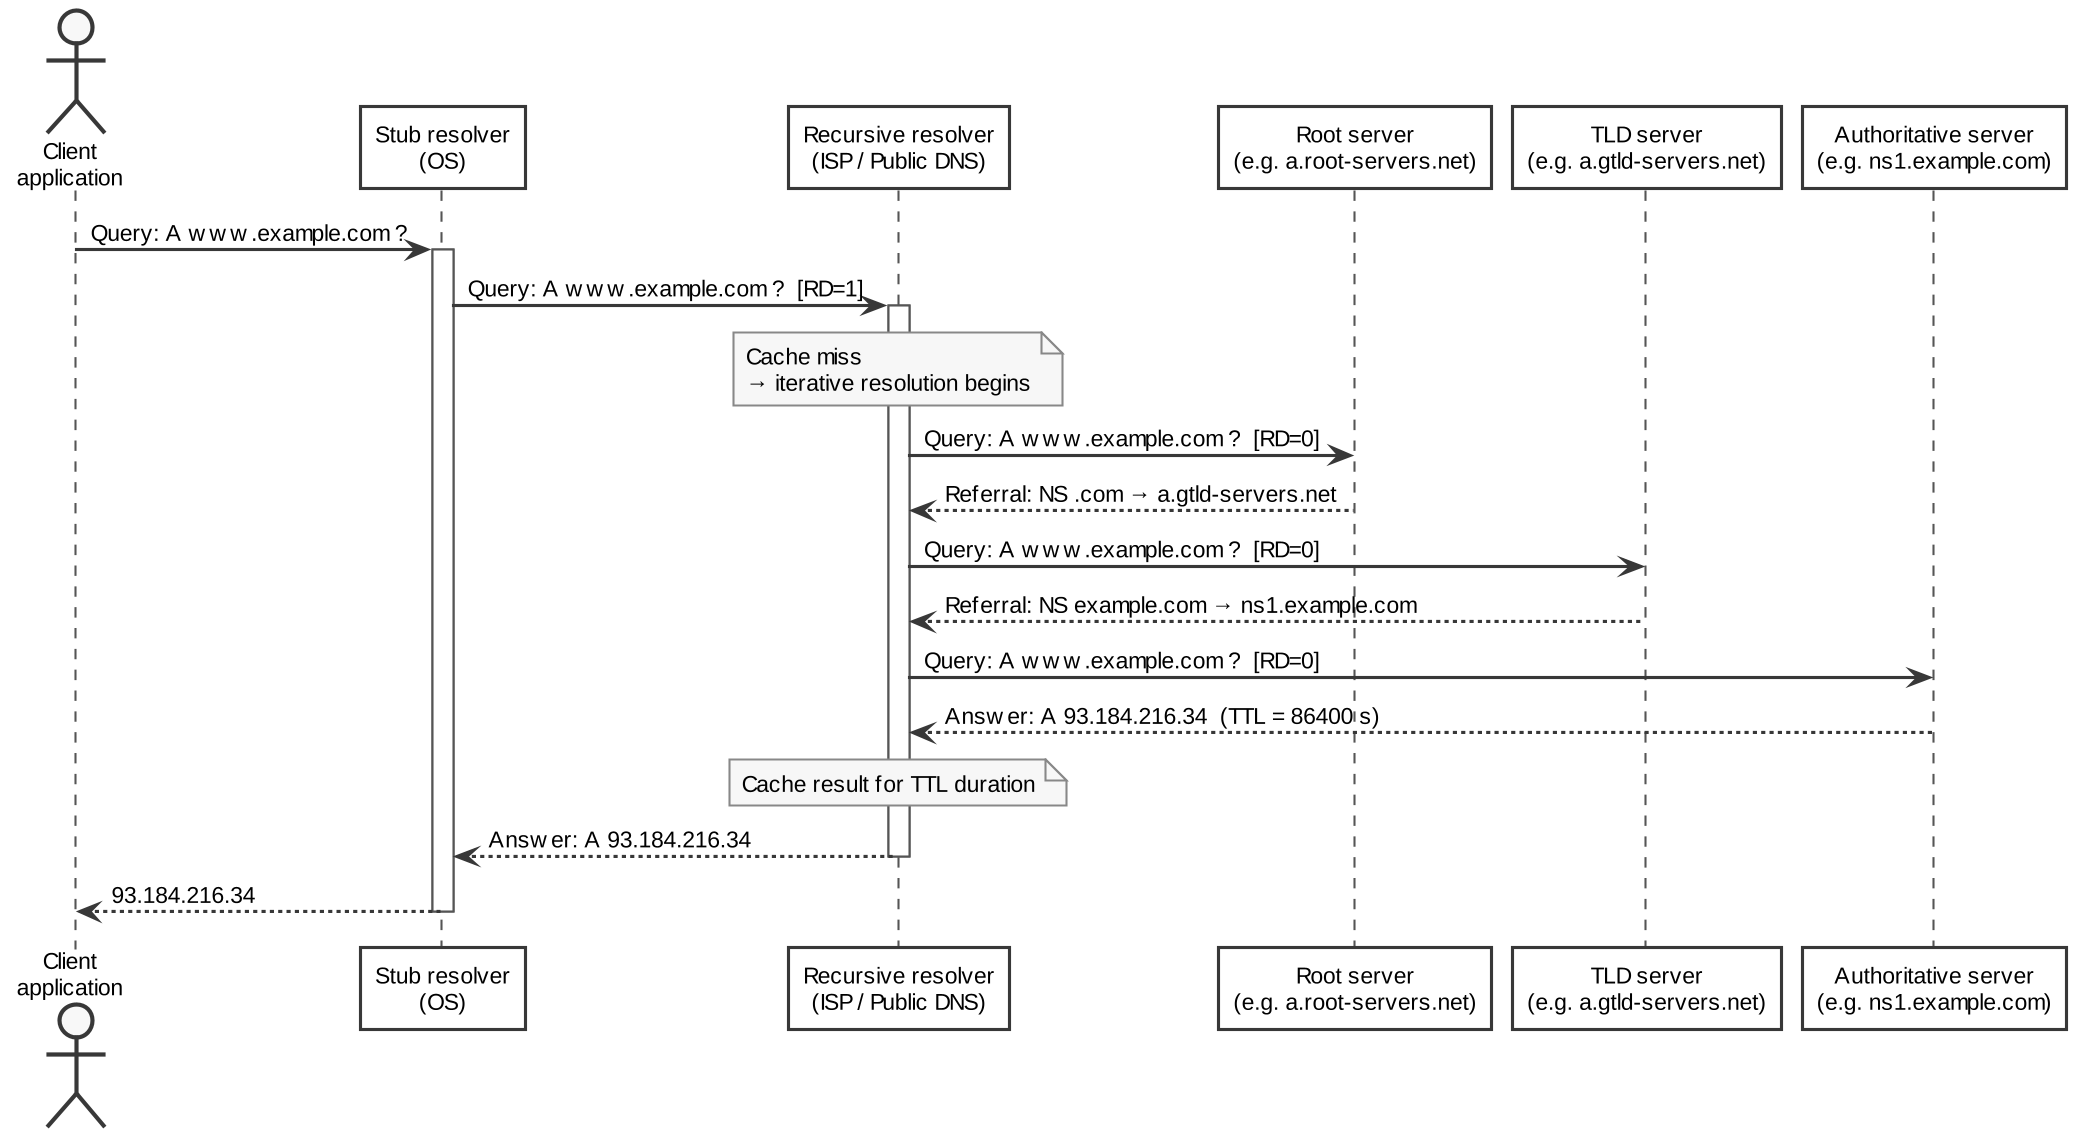
\includegraphics[width=0.92\linewidth]{figures/fig1_dns_resolution.png}
  \caption{Iterative \ac{DNS} resolution process. The client-side resolver (stub) forwards the query to a recursive resolver, which performs three successive referral queries (root $\rightarrow$ \ac{TLD} $\rightarrow$ authoritative) before returning the final answer. The \ac{TTL} field in the authoritative response governs how long the recursive resolver caches the result.}
  \label{fig:DNS_resolution}
\end{figure}

There is a wrinkle. Route a Namur probe through Google 8.8.8.8 and the \ac{CDN} sees Mountain View, California — not Belgium. It assigns a California-region server. The probe is in the wrong region for its own query. RIPE Atlas sidesteps this by querying authoritative servers with the \ac{RD} bit unset. The query arrives from the probe's own Belgian \ac{IP}. The \ac{CDN} routes accordingly. Q4 deliberately breaks that assumption to measure what changes when resolver choice overrides probe location.

\bigskip
\section{Research Questions and Objectives}
\label{sec:1.3}

This thesis addresses the following main research question:

\textit{How can one design and deploy a distributed \ac{DNS} measurement system that captures the geographic and temporal diversity of \ac{DNS} responses for the most popular domains on the web, in a manner that is ethically sound, reproducible, and useful to the research community?}

The main question decomposes into four:

Q1 --- \textit{Geographic diversity}: What share of popular domains return different \ac{DNS} responses depending on where the query originates? For those that do, which mechanism accounts for it — \ac{CDN} routing policy, anycast topology, or \ac{ECS}?

RIPE Atlas accounts are subject to a cap on concurrent measurements. Working through the Tranco Top-10K would require roughly 10,000 measurements running simultaneously — far beyond typical limits. Top-250 is where the budget runs out. That constraint matters less than it might seem: geographic \ac{DNS} routing via \ac{CDN} is concentrated among the highest-traffic domains anyway.

Q2 --- \textit{Temporal stability}: What is the temporal stability of \ac{DNS} responses at day, week, and month timescales over the measurement period?

Q3 --- \textit{RIPE Atlas geographic bias}: Do the documented geographic biases of the RIPE Atlas probe distribution~\cite{Bajpai2017} (91\% of probes in Europe/North America) significantly affect the ability to observe \ac{DNS} geographic variation?

Q4 --- \textit{Resolver impact}: Does switching from a local \ac{ISP} resolver to Google 8.8.8.8 or Cloudflare 1.1.1.1 change the \ac{DNS} answer a probe receives? Does that difference interact with where the probe is located?

Fifty days, one measurement per day: 2~April through 21~May~2026. A pilot phase (02--09~April, 99~domains, 50~probes) confirmed the fetch-and-parse pipeline before the main campaign scaled to 250~domains $\times$ 200~probes on 11~April. Each morning a cron job fetched the previous day's results from the RIPE Atlas \ac{API} and parsed them into dated Parquet files on a Raspberry Pi at home, synced nightly to Google Drive. Q4 did not run as planned: RIPE Atlas enforces a cap of 100 concurrent one-off measurements per account, and with 247~periodic measurements already active, no slot was available for the resolver-comparison campaign. The three completed questions draw from the same authoritative-side dataset.

\bigskip
\section{Thesis Structure}
\label{sec:1.4}

Chapter~\ref{ch:state-of-the-art} reviews distributed \ac{DNS} measurement, geographic routing, and probe bias, and locates this thesis within that literature. Chapter~\ref{ch:method} covers corpus selection, probe configuration, and the collection pipeline. Chapter~\ref{ch:results} presents measurements for Q1--Q3 along with partial Q4 data. Chapter~\ref{ch:conclusion} interprets the findings and identifies what remains open.
